There are two decompositions that are used extensively in this thesis: The QR-decomposition and the Singular Value Decomposition. Both decompositions are matrix decompositions but can be applied to tensors as well by first grouping indices and reshaping to a matrix, applying the decomposition, and reshaping the result back to the original indices. \par
The \textit{reduced QR-decomposition} of a matrix $A \in \mathbb{C}^{n\times m}$ is the decomposition
\begin{equation}
	\label{eq:QR_decomposition_general}
	A = QR,
\end{equation}
where $Q\in\mathbb{C}^{n\times k}$ is an isometry, $R\in\mathbb{C}^{k\times m}$ is an upper triangular matrix and $k \coloneqq \min(n, m)$. The computational complexity of the QR decomposition scales as
\begin{equation}
	\label{eq:QR_decomposition_complexity}
	\mathcal{O}\left(nmk\right).
\end{equation}
The QR decomposition is drawn as a tensor diagram in Figure \figref{fig:tensor_decomposition_qr}. \par
The \textit{Singular Value Decomposition} (SVD) of a matrix $A \in \mathbb{C}^{n\times m}$ is the decomposition
\begin{equation}
	\label{eq:SVD_general}
	A = USV^\dagger,
\end{equation}
where $U\in\mathbb{C}^{n\times k}$ and $V\in\mathbb{C}^{m\times k}$ are isometries, $S\in\mathbb{R}^{k\times k}$ is a diagonal real matrix of non-negative \textit{singular values}, and $k \coloneqq \min(n, m)$. The computational complexity of the SVD is the same as for the QR decomposition \eqref{eq:QR_decomposition_complexity}. However, while the scaling is the same, the prefactors are lower for the QR decomposition in most implementations, meaning that the QR decomposition is faster in practice. Moreover, in contrast to the SVD, the QR decomposition allows for highly efficient implementations on graphics processing units (GPUs), which enables decompositions of large matrices to be carried out significantly faster and more power efficiently. Thus, whenever the singular values are not needed, the QR decomposition is preferred over the SVD. Figure \figref{fig:tensor_decomposition_svd} shows a tensor network diagram of the SVD \eqref{eq:SVD_general}. \par
An important property of the SVD is that it can be used to approximate a matrix $A$ by a matrix $\tilde{A}$ of lower rank $\chi < \min(m, n)$. This \textit{truncated SVD} can be performed by keeping only the largest $\chi < k$ singular values and omitting the corresponding columns of $U$ and $V$:
\begin{equation}
	\label{eq:truncated_SVD_general}
	A \approx \tilde{A} = \tilde{U}\tilde{S}\tilde{V},
\end{equation}
with isometries $\tilde{U}\in\mathbb{C}^{n\times\chi}$, $\tilde{V}\in\mathbb{C}^{m\times\chi}$ and real diagonal matrix $\tilde{S}\in\mathbb{C}^{\chi\times\chi}$ with non-negative entries. It can be shown \cite{cite:eckart_young_theorem} that the truncated SVD minimizes the distance $\lVert A - \tilde{A} \rVert_\text{F}$ between $A$ and $\tilde{A}$ under the constraint $\text{rank}(\tilde{A}) = \chi$. The remaining \textit{truncation error} is
\begin{equation}
	\varepsilon_\text{trunc} = \lVert A - \tilde{A} \rVert_\text{F} = \sqrt{\sum_{i=\chi+1}^{\min(m,n)} S_i^2},
\end{equation} 
where we have sorted the singular values in descending order. The truncated SVD is frequently used in tensor network algorithms to truncate tensors to a maximum bond dimension $\chi_\text{max}$. \par
\begin{figure}
	\centering
	\begin{subfigure}[c]{0.1\textwidth}
		\caption{}\label{fig:tensor_decomposition_qr}
	\end{subfigure}%
	\begin{minipage}[c]{0.6\textwidth}
		\raisebox{-26pt}
		{%
			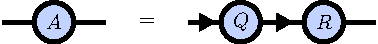
\includegraphics[scale=1]{figures/tikz/Tensor_Networks/tensor_decompositions/tensor_decompositions_a.pdf}
		}
	\end{minipage}
	\par\medskip
	\begin{subfigure}[c]{0.1\textwidth}
		\caption{}\label{fig:tensor_decomposition_svd}
	\end{subfigure}%
	\begin{minipage}[c]{0.6\textwidth}
		\raisebox{-26pt}
		{%
			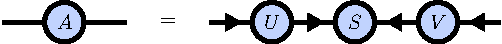
\includegraphics[scale=1]{figures/tikz/Tensor_Networks/tensor_decompositions/tensor_decompositions_b.pdf}
		}
	\end{minipage}
	\caption{Tensor decompositions are shown in tensor network diagram notation. (a) QR-decomposition \eqref{eq:QR_decomposition_general}. (b) Singular Value Decomposition \eqref{eq:SVD_general}}
	\label{fig:tensor_decomposition_diagrams}
\end{figure}